\documentclass[tikz]{standalone}
\usepackage{pgfplots}
\usepackage{mathtools}
\pgfplotsset{compat = newest}
\definecolor{lessgreen}{RGB}{0,150,0}

\pgfdeclareverticalshading{rainbow}{100bp}
{color(0bp)=(red); color(25bp)=(red); color(35bp)=(yellow);
color(45bp)=(green); color(55bp)=(cyan); color(65bp)=(blue);
color(75bp)=(violet); color(100bp)=(violet)}

\begin{document}
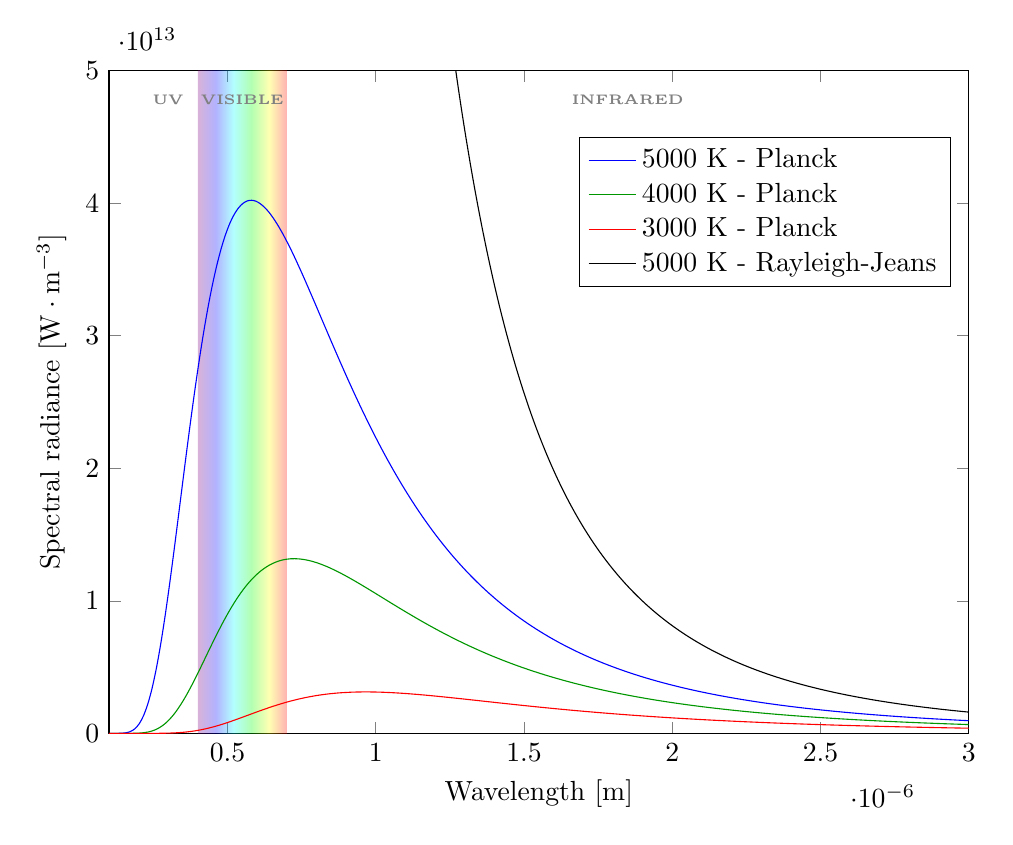
\begin{tikzpicture}
  \def\c{299792458}
  \def\h{6.626070*10^(-34)}
  \def\kb{1.380649*10^(-23)}
  \begin{axis}[
      width=12.5cm,
      height=10cm,
      xmin = 1e-7,
      xmax = 3e-6,
      %xtick distance = 0.001,
      ymin = -1e10,
      ymax = 5e13,
      % axis equal image,
      ylabel={Spectral radiance [$\text{W}\cdot\text{m}^{-3}$]},
      xlabel={Wavelength [m]},
      legend cell align = {left}, %
      legend style={at={(axis cs:2.94e-6,4.5e13)},anchor=north east} % position of the legend box and anchor is the point on the box to be fitted exactly at the point of cs:<>,<>. Options are anchor=center,south west,south east,north west,north east,north,south,west...
    ]
    \shade[shading=rainbow,shading angle=90,opacity=0.3] (axis cs:400e-9,0) rectangle (axis cs:700e-9,5e13);
    \node[font=\tiny, black!50] at (axis cs: 300e-9,4.78e13) {\textbf{UV}};
    \node[font=\tiny, black!50] at (axis cs: 550e-9,4.78e13) {\textbf{VISIBLE}};
    \node[font=\tiny, black!50] at (axis cs: 1850e-9,4.78e13) {\textbf{INFRARED}};

    % Planck
    \addplot [thin,samples=200,smooth,blue,domain=1e-7:3e-6] {2*pi*\h*\c*\c/(x^5*(e^(\h*\c/(x*\kb*5000))-1))}; % 5000 K
    \addplot [thin,samples=200,smooth,lessgreen,domain=1e-7:3e-6] {2*pi*\h*\c*\c/(x^5*(e^(\h*\c/(x*\kb*4000))-1))}; % 4000 K
    \addplot [thin,samples=200,smooth,red,domain=1e-7:3e-6] {2*pi*\h*\c*\c/(x^5*(e^(\h*\c/(x*\kb*3000))-1))}; % 3000 K
    % Rayleigh-Jeans
    \addplot [thin,samples=200,smooth,black,domain=1.25e-6:3e-6] {2*pi*\c*\kb*5000/x^4}; % 5000 K
    \legend{5000 K - Planck,4000 K - Planck,3000 K - Planck,5000 K - Rayleigh-Jeans}
  \end{axis}
\end{tikzpicture}
\end{document}